\documentclass{beamer}

\usepackage{beamerthemesplit}

\usepackage[T1]{fontenc}
\usepackage[thai]{babel}
\usepackage{setspace}
\usepackage{color}
\usepackage[utf8x]{inputenc}
\usepackage{array} % for \arraybackslash}m in table.

\usepackage{epstopdf}\usepackage{fancyvrb} % to allow small font verbatim

\usepackage{listings}

\usepackage{xcolor}
\newcommand{\highlight}[1]{%
  \colorbox{yellow!50}{$\displaystyle#1$}}

\usepackage{graphicx} % for background image

%\usetheme{Antibes}
%\usetheme{Szeged}
%\usetheme{CambridgeUS}
%\usetheme{Warsaw}

%\setbeamertemplate{headline}
%{%
%  \begin{beamercolorbox}[ht=3ex,dp=2ex]{section in head/foot}%
%    \insertnavigation{\paperwidth}
%  \end{beamercolorbox}%
%}%

%\setbeamertemplate{footline}
%{%
%  \begin{beamercolorbox}[ht=3ex,dp=2ex]{section in head/foot}%
% Date \insertshortdate
% \insertshorttitle
% Page \insertpagenumber
%  \end{beamercolorbox}%
%}%

\usepackage{textpos} % for textblock (adding KKU logo) May 31st, 2018.


\setbeamertemplate{bibliography item}{\insertbiblabel}
% for numbered bib. Jan 19th, 2018.

\definecolor{KKU1}{RGB}{217, 76, 31}

\definecolor{COCO1}{RGB}{239, 60, 34}
\definecolor{COCO2}{RGB}{249, 159, 28}
\definecolor{COCO3}{RGB}{239, 80, 159}
\definecolor{COCO4}{RGB}{35, 152, 203}
\definecolor{COCO5}{RGB}{173, 161, 52}

\definecolor{G1}{RGB}{35, 152, 103}
\definecolor{G2}{RGB}{0, 128, 0}

\definecolor{LightGray}{RGB}{210, 210, 210}

\definecolor{BlueGreen}{RGB}{40, 255, 255}


\definecolor{TreeBrown}{RGB}{162, 64, 17}

\setbeamercolor{title}{fg=white,bg=KKU1}

\setbeamercolor*{palette primary}{use=structure,fg=white,bg=G2}
\setbeamercolor*{palette secondary}{use=structure,fg=white,bg=TreeBrown}
\setbeamercolor*{palette tertiary}{use=structure,fg=yellow,bg=TreeBrown}
\setbeamercolor*{palette quaternary}{fg=white,bg=COCO5}


\usetheme{Madrid}

\setbeamertemplate{footline}
{%
\vskip-9ex%
\pgfsetfillopacity{0}\begin{beamercolorbox}{}
\hfill\usebeamercolor[COCO1]{}
%navigation symbols}%
	\pgfsetfillopacity{1}
%    \insertslidenavigationsymbol
%    \insertframenavigationsymbol
%    \insertsubsectionnavigationsymbol
    \insertsectionnavigationsymbol
%    \insertdocnavigationsymbol
%    \insertbackfindforwardnavigationsymbol
    \hspace{1em}%
    \insertframenumber/\inserttotalframenumber   
    \hspace{1em} 
  \end{beamercolorbox}%    
\pgfsetfillopacity{0}
\begin{beamercolorbox}[ht=3ex,dp=4ex]{section in head/foot}%
	\pgfsetfillopacity{1}
%    \insertnavigation{\paperwidth}
    \insertsectionnavigationhorizontal{\paperwidth}{}{}
  \end{beamercolorbox}
}%

% Set verbatim font. Dec 26th, 2017.
\usepackage{verbatim}% http://ctan.org/pkg/verbatim
\makeatletter
\newcommand{\verbatimfont}[1]{\def\verbatim@font{#1}}%
\makeatother

%\usepackage{inconsolata}
\verbatimfont{\itshape\ttfamily\color{blue}}
%\usepackage{fontspec}
%\setmonofont{Consolas}



\title{Linear Circuit Analysis:\\
Ch 11, AC Steady State Power}
\author{Tatpong Katanyukul}
\institute{\vspace{-0.2in}\includegraphics[height=0.5cm]{../shared/long-logo-color.png}}
\date{\today}

\lstset{
  language=Python,
  basicstyle=\ttfamily\scriptsize,
  breaklines=true,
  prebreak=\raisebox{0ex}[0ex][0ex]{\ensuremath{\hookleftarrow}},
  frame=lines,
  showtabs=false,
  showspaces=false,
  showstringspaces=false,
  keywordstyle=\color{blue},
  stringstyle=\color{green!50!black},
  commentstyle=\color{gray}\itshape,
  numbers=left,
  numbersep=5pt,
  captionpos=t,
  escapeinside={(*}{*)}
}

\addtobeamertemplate{frametitle}{
}{%

\begin{textblock*}{100mm}(-0.4cm,-1.5cm)
\includegraphics[height=1.8cm]{../shared/overlay.png}
\end{textblock*}

\begin{textblock*}{100mm}(0.92\textwidth,-1.1cm)
\includegraphics[height=1.2cm]{../shared/glowingKKU.png}
\end{textblock*}
}

\addtobeamertemplate{footline}{
\begin{textblock*}{100mm}(0cm,-0.6cm)
\includegraphics[width=7in]{../shared/teak.png}
\end{textblock*}{}
}


%%%%%%%%%%%%%%%%%%%%%%%%%%%%%%%%%%%%%%%%%%%%%%%%%%%%%%%%

\begin{document}

{
\setbeamertemplate{footline}{} % omit footline on the 
\begin{frame}
  \titlepage
\end{frame}
}%
%%%%%%%%%%%%%%%%%%%%%%%%%%%%%%%%%%%

\begin{frame}[fragile]

\frametitle{Key Concepts}

Key Concepts:
\begin{itemize}
\item Instantaneous power
\item Average power
\item Effective or rms values
\item Complex power
\item Power factor
\item Power factor correction
\end{itemize}

\end{frame}
%%%%%%%%%%%%%%%%%%%%%%%%%%%%%%%%%%%

\begin{frame}[fragile]
\frametitle{Recall an AC Steady-State System}

\begin{center}
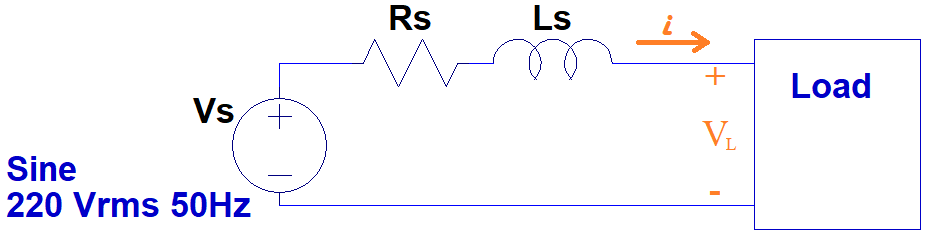
\includegraphics[width=2.65in]{src/Fig01b.png}
\end{center}

\begin{itemize}
\item $V_L = i \cdot Z_{\rm{Load}}$
\end{itemize}

\begin{center}
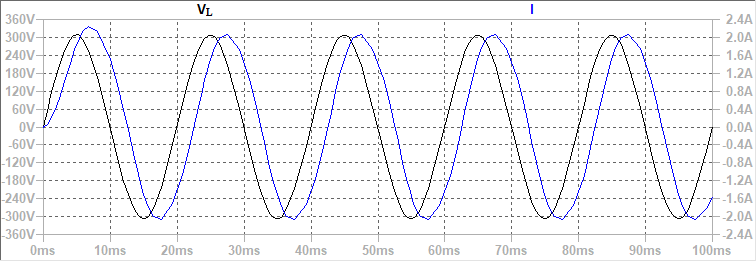
\includegraphics[width=2.65in]{src/Fig02b.png}
\end{center}

\end{frame}

%%%%%%%%%%%%%%%%%%%%%%%%%%%%%%%%%%%

\section{Instantaneous power}

\begin{frame}[fragile]
\frametitle{Instantaneous Power}

\begin{center}
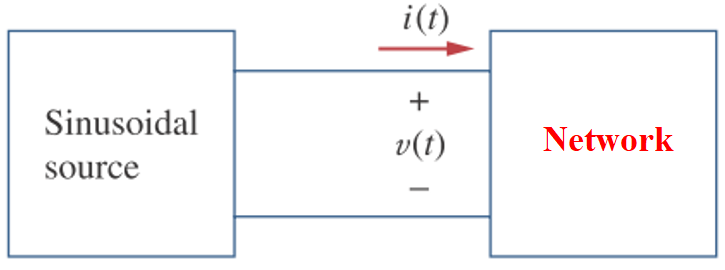
\includegraphics[width=2.65in]{src/Fig03a.png}
\end{center}

Instantaneous power:
\begin{itemize}
\item Instantaneous power is a power at a particular point in time.
\item $p(t) = v(t) \cdot i(t)$
\\ where $v(t)$ and $i(t)$ are voltage and current at the particular time. 
\item When $p(t) > 0$, the network is consuming power.
\item When $p(t) < 0$, the network in supplying power.
\end{itemize}

\end{frame}

%%%%%%%%%%%%%%%%%%%%%%%%%%%%%%%%%%%

\begin{frame}[fragile]
\frametitle{Instantaneous Power of an AC System (I)}

\begin{center}
$p(t) = v(t) \cdot i(t)$
\end{center}

\begin{center}
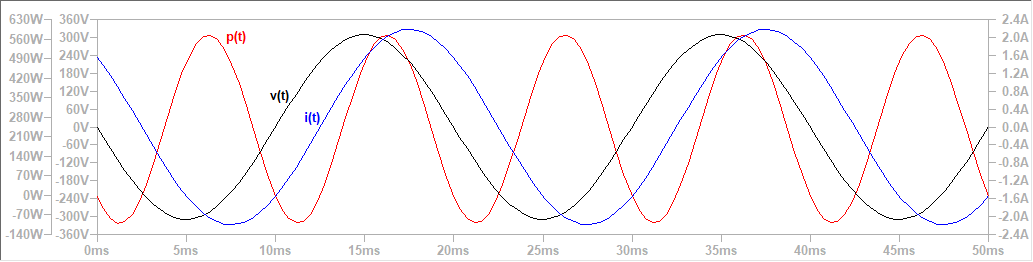
\includegraphics[width=0.8\textwidth]{src/Fig04a.png}
\end{center}

Given $v(t) = V_m \cos(\omega t + \theta_V)$ 
and $i(t) = I_m \cos(\omega t + \theta_I)$,
%
\begin{eqnarray}
p(t) &=& V_m \cos(\omega t + \theta_V) \cdot I_m \cos(\omega t + \theta_I)
\nonumber \\
&=& V_m I_m \cos(\omega t + \theta_V) \cdot \cos(\omega t + \theta_I)
\nonumber .
\end{eqnarray}

\end{frame}

%%%%%%%%%%%%%%%%%%%%%%%%%%%%%%%%%%%

\begin{frame}[fragile]
\frametitle{Instantaneous Power of an AC System (II)}

\vspace{-1cm}

\begin{eqnarray}
p(t) &=& V_m I_m \cos(\omega t + \theta_V) \cdot \cos(\omega t + \theta_I)
\nonumber .
\end{eqnarray}

From a product of cosine identity: $\cos(A )\cos(B) = \frac{1}{2} \left\{ \cos(A-B) + \cos(A+B) \right\}$, 
therefore\\
\begin{eqnarray}
p(t) &=& \frac{V_m I_m}{2} \left\{ 
\cos(\theta_V - \theta_I)  + \cos(2 \omega t + \theta_V + \theta_I)
\right\}
\nonumber \\
&=& \underbrace{\frac{V_m I_m}{2} \cos(\theta_V - \theta_I)}_{\mbox{time-constant part}} + \underbrace{\frac{V_m I_m}{2} \cos(2 \omega t + \theta_V + \theta_I)}_{\mbox{time-varying part}}
\label{eq: ac instantaneous power} .
\end{eqnarray}

\end{frame}

%%%%%%%%%%%%%%%%%%%%%%%%%%%%%%%%%%%

\begin{frame}[fragile]
\frametitle{Instantaneous Power of an AC System (III)}

\vspace{-1cm}

\begin{eqnarray}
p(t) &=& \underbrace{\frac{V_m I_m}{2} \cos(\theta_V - \theta_I)}_{\mbox{offset}} + \underbrace{\frac{V_m I_m}{2} \cos(2 \omega t + \theta_V + \theta_I)}_{\mbox{sinusoid}}
\nonumber .
\end{eqnarray}
%
\begin{center}
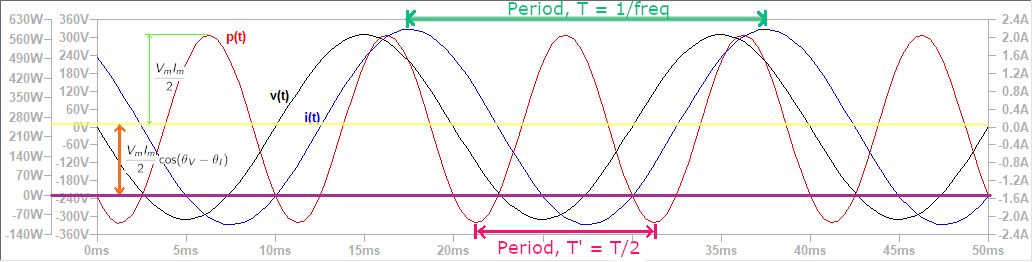
\includegraphics[width=0.8\textwidth]{src/Fig05a.png}
\end{center}

\begin{itemize}
\item $\frac{V_m I_m}{2} \cos(\theta_V - \theta_I)$ (constant to time) plays an offset role.
\item $\frac{V_m I_m}{2} \cos(2 \omega t + \theta_V + \theta_I)$ is a sinusoidal part with its frequency doubled from the original.
\\ $\Rightarrow$ its magnitude is $\frac{V_m I_m}{2}$.
\end{itemize}


\end{frame}

%%%%%%%%%%%%%%%%%%%%%%%%%%%%%%%%%%%

\begin{frame}[fragile]
\frametitle{Recall Properties of R, L, and C}

\vspace{-1cm}

\begin{itemize}
\item R: $\mathbb{I} =\mathbb{V}/R = \frac{V_m}{R} \angle \theta_V$ 
\\
$\Rightarrow$ $I$ and $V$ are in phase: $\theta_V = \theta_I$.
\item L: $\mathbb{I} = \mathbb{V}/(j \omega L) = = \frac{V_m}{\omega L} \angle (\theta_V - \frac{\pi}{2})$ 
\\
$\Rightarrow$ $I$ lags $V$ by $\frac{\pi}{2}$: $\theta_V - \theta_I = \frac{\pi}{2}$.
\item C: $\mathbb{I} = \mathbb{V} \cdot (j \omega C) = = V_m \omega C \angle (\theta_V + \frac{\pi}{2})$ 
\\
$\Rightarrow$ $I$ leads $V$ by $\frac{\pi}{2}$: $\theta_V - \theta_I = -\frac{\pi}{2}$.
\end{itemize}

\end{frame}

%%%%%%%%%%%%%%%%%%%%%%%%%%%%%%%%%%%

\begin{frame}[fragile]
\frametitle{Instantaneous Power on R, L, and C (I)}

\vspace{-1cm}

\begin{eqnarray}
p(t) &=& \underbrace{\frac{V_m I_m}{2} \cos(\theta_V - \theta_I)}_{\mbox{offset}} + \underbrace{\frac{V_m I_m}{2} \cos(2 \omega t + \theta_V + \theta_I)}_{\mbox{sinusoid}}
\nonumber .
\end{eqnarray}
%
\begin{tabular}{|l|l|l|}
\hline
R: In phase & L: Lagging by $\frac{\pi}{2}$ & C: Leading by $\frac{\pi}{2}$ \\
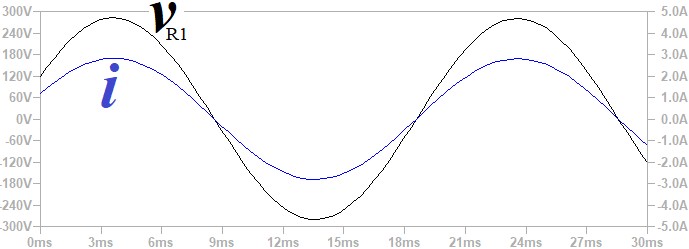
\includegraphics[width=0.3\textwidth]{src/FigRLC_inphase.png}
&
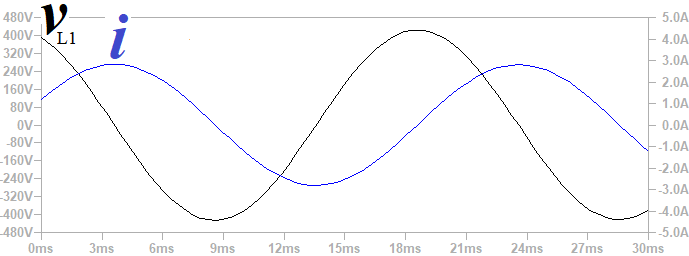
\includegraphics[width=0.3\textwidth]{src/FigRLC_lagging.png}
&
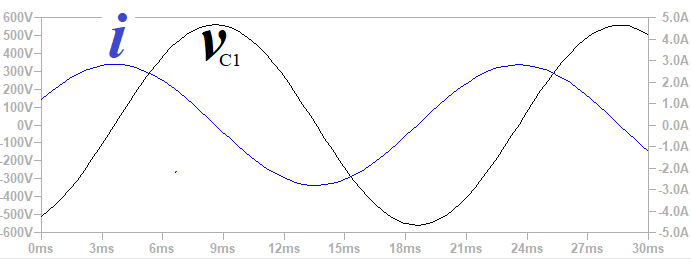
\includegraphics[width=0.3\textwidth]{src/FigRLC_leading.png}
\\
$\theta_V = \theta_I$ 
& 
$\theta_V - \theta_I = \frac{\pi}{2}$ 
& 
$\theta_V - \theta_I = -\frac{\pi}{2}$
\\
$\Rightarrow$ offset = $\frac{V_m I_m}{2}$.
&
$\Rightarrow$ offset = $0$.
&
$\Rightarrow$ offset = $0$.
\\
\hline
With this offset, 
&
\multicolumn{2}{l|}{With no offset, }
\\
$p_R \geq 0$ all the times.
&
\multicolumn{2}{l|}{sinusoid will oscillate around $0$.}
\\ \hline
\end{tabular}

\end{frame}

%%%%%%%%%%%%%%%%%%%%%%%%%%%%%%%%%%%

\begin{frame}[fragile]
\frametitle{Instantaneous Power on R, L, and C (II)}

\vspace{-1cm}

\begin{eqnarray}
p(t) &=& \frac{V_m I_m}{2} \cos(\theta_V - \theta_I) + \frac{V_m I_m}{2} \cos(2 \omega t + \theta_V + \theta_I)
\nonumber .
\end{eqnarray}
%
\begin{tabular}{|l|l|l|}
\hline
R: In phase & L: Lagging & C: Leading \\
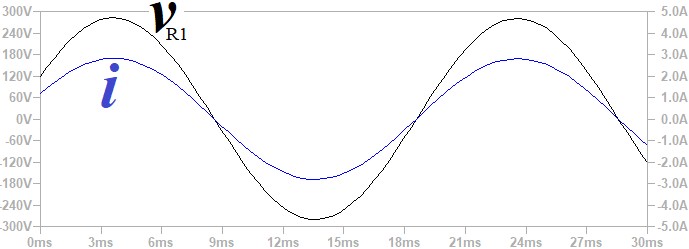
\includegraphics[width=0.3\textwidth]{src/FigRLC_inphase.png}
&
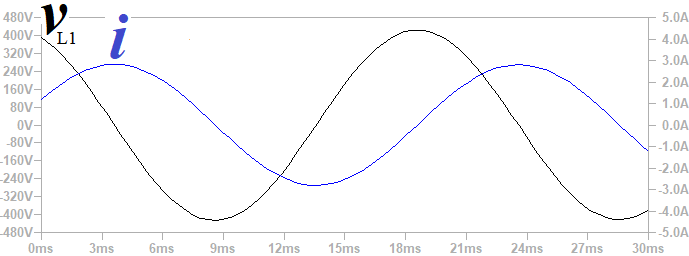
\includegraphics[width=0.3\textwidth]{src/FigRLC_lagging.png}
&
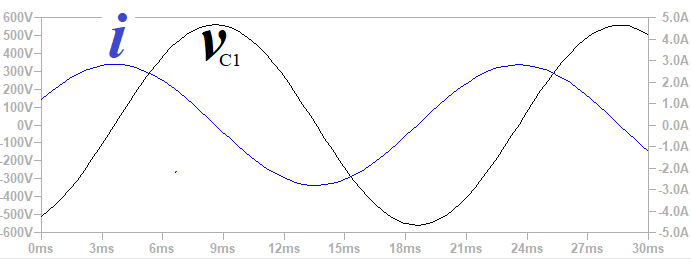
\includegraphics[width=0.3\textwidth]{src/FigRLC_leading.png}
\\
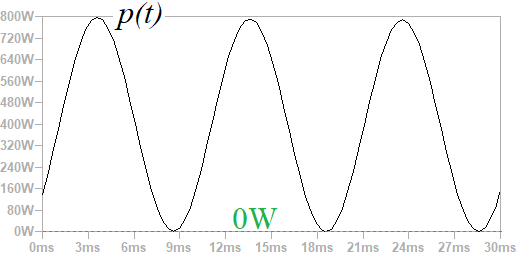
\includegraphics[width=0.3\textwidth]{src/FigPower_inphase.png}
&
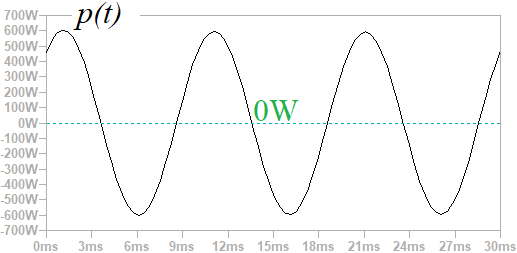
\includegraphics[width=0.3\textwidth]{src/FigPower_lagging.png}
&
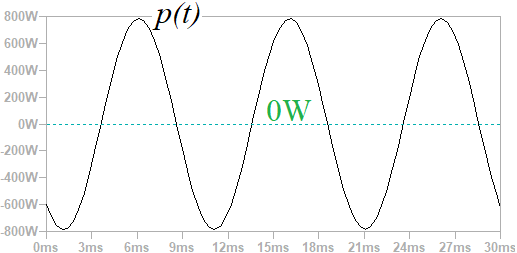
\includegraphics[width=0.3\textwidth]{src/FigPower_leading.png}
\\ \hline
offset = $\frac{V_m I_m}{2}$.
&
\multicolumn{2}{c|}{offset = $0$. }
\\
$p(t) \geq 0$ always.
&
\multicolumn{2}{c|}{$p(t) \geq 0$ half the times }
\\
&
\multicolumn{2}{c|}{$p(t) \leq 0$ another half }
\\ \hline
\end{tabular}

\end{frame}

%%%%%%%%%%%%%%%%%%%%%%%%%%%%%%%%%%%

\begin{frame}[fragile]
\frametitle{Instantaneous Power on R, L, and C (III)}

\vspace{-1cm}

\begin{tabular}{|l|l|l|}
\hline
R: In phase & L: Lagging & C: Leading \\
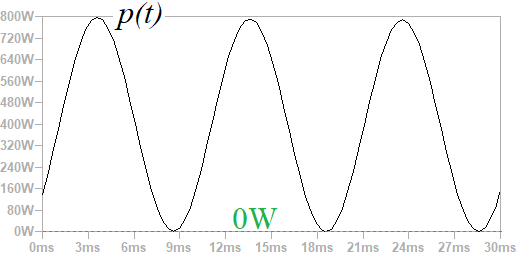
\includegraphics[width=0.3\textwidth]{src/FigPower_inphase.png}
&
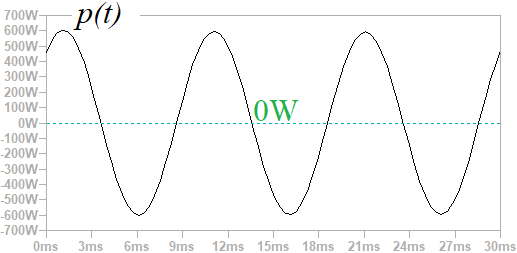
\includegraphics[width=0.3\textwidth]{src/FigPower_lagging.png}
&
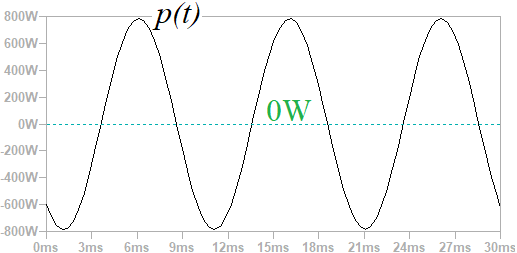
\includegraphics[width=0.3\textwidth]{src/FigPower_leading.png}
\\ \hline
$p(t) \geq 0$ always.
&
\multicolumn{2}{c|}{$p(t) \geq 0$ half the times }
\\
&
\multicolumn{2}{c|}{$p(t) \leq 0$ another half }
\\ \hline
R always consumes
&
\multicolumn{2}{l|}{L and C are energy-storage devices.}
\\
power.
&
\multicolumn{2}{l|}{$p(t) > 0 \Rightarrow$ stores power}
\\
&
\multicolumn{2}{l|}{$p(t) < 0 \Rightarrow$ releases power}
\\ \hline
\end{tabular}

\end{frame}

%%%%%%%%%%%%%%%%%%%%%%%%%%%%%%%%%%%


\begin{frame}[fragile]
\frametitle{Example: Instantaneous Power (I)}

\vspace{-1cm}

\begin{columns}[c]
\column{0.4\textwidth}

\begin{center}
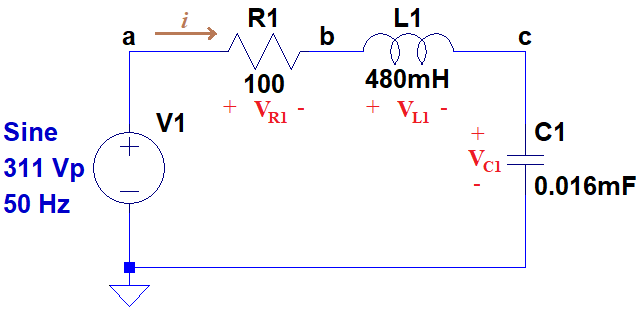
\includegraphics[width=\textwidth]{src/Fig06a.png}
\end{center}
%
\vspace{-0.5cm}
%
\begin{itemize}
\item $V_1(t) = 311 \sin(314.2 t)$
\item $\mathbb{V}_1 \equiv 311 \angle -\frac{\pi}{2}$
\item $\mathbb{Z}_{R1} = 100 \Omega$ 
\item $\mathbb{Z}_{L1} = j150.8 \Omega$
\item $\mathbb{Z}_{C1} = -j198.9 \Omega$
\item $\mathbb{Z} = 100 -j48.1 \Omega$ 
\end{itemize}

\column{0.58\textwidth}

\begin{itemize}
\item $\therefore \mathbb{I} = \mathbb{V}_1/\mathbb{Z} = 2.8 \angle -1.12$
%(flowing direction: a to b)
\item $i(t) = 2.8 \cos(314.2 t - 1.12)$
\item $\mathbb{V}_{R1} = \mathbb{I} \cdot \mathbb{Z}_{R1} = 280.3 \angle -1.12$
\item $\mathbb{V}_{L1} = \mathbb{I} \cdot \mathbb{Z}_{L1} = 422.6 \angle 0.45$
\item $\mathbb{V}_{C1} = \mathbb{I} \cdot \mathbb{Z}_{C1} = 557.4 \angle -2.69$
\item $V_{R1}(t) = 280.3 \cos(314.2 t - 1.12)$
\item $V_{L1}(t) = 422.6 \cos(314.2 t + 0.45)$
\item $V_{C1}(t) = 557.4 \cos(314.2 t - 2.69)$
\end{itemize}

%\begin{verbatim}[fontsize=\small]
%* RLC Power
%V1 a 0 SINE(0 311 50)
%R1 b a 100
%L1 b c 480mH
%C1 c 0 0.016mF
%.tran 0 1.06 1 200
%.end
%\end{verbatim}



\end{columns}


\end{frame}

%%%%%%%%%%%%%%%%%%%%%%%%%%%%%%%%%%%

\begin{frame}[fragile]
\frametitle{Example: Instantaneous Power (II)}

\vspace{-1cm}

\begin{flushright}
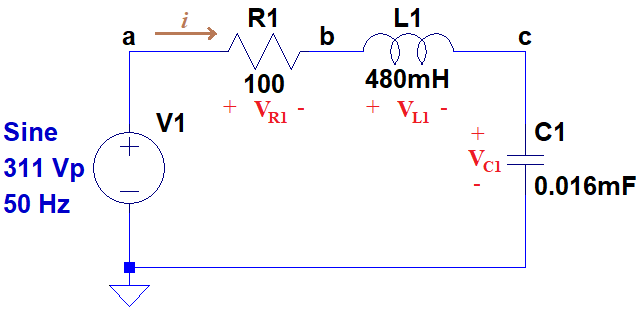
\includegraphics[width=0.4\textwidth]{src/Fig06a.png}
\end{flushright}

\vspace{-1cm}

\begin{itemize}
\item $I_m = 2.8$; $\theta_I = -1.12$
\item $V_m(R1) = 280.3$; $\theta_V(R1) = -1.12$
\item $V_m(L1) = 422.6$; $\theta_V(L1) = 0.45$
\item $V_m(C1) = 557.4$; $\theta_V(C1) = -2.69$
%
\item $p_{R1}(t) = \frac{(280.3)(2.8)}{2} + \frac{(280.3)(2.8)}{2} \cos( 2(314.2)t -1.12 - 1.12)$
\item $p_{L1}(t) = \frac{(422.6)(2.8)}{2} \cos( 2(314.2)t + 0.45 -1.12)$
\item $p_{C1}(t) = \frac{(557.4)(2.8)}{2} \cos( 2(314.2)t -2.69 -1.12)$
\end{itemize}


\end{frame}

%%%%%%%%%%%%%%%%%%%%%%%%%%%%%%%%%%%

\begin{frame}[fragile]
\frametitle{Example: Instantaneous Power (III)}

\vspace{-1cm}
\begin{center}
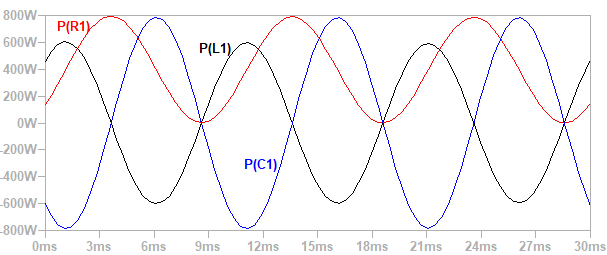
\includegraphics[width=0.5\textwidth]{src/Fig07a.png}
\end{center}

\begin{itemize}
\item $p_{R1}(t) = 392.4 + 392.4 \cos(628.4 t -2.24)$
\item $p_{L1}(t) = 591.6 \cos(628.4 t - 0.67)$
\item $p_{C1}(t) = 780.4 \cos(628.4 t - 3.81)$
\end{itemize}

\end{frame}

%%%%%%%%%%%%%%%%%%%%%%%%%%%%%%%%%%%


\begin{frame}[fragile]
\frametitle{Example: Instantaneous Power (IV)}

\vspace{-0.5cm}
\begin{columns}[c]
\column{0.475\textwidth}
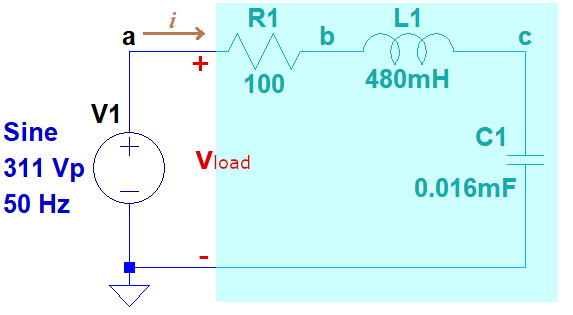
\includegraphics[width=0.75\textwidth]{src/Fig08a.png}

\column{0.475\textwidth}
\includegraphics[width=\textwidth]{src/FigPower_load.png}

\end{columns}

\begin{itemize}
\item $V_{\mbox{load}} = V_1$ 
\\
$\Rightarrow$ $\therefore \mathbb{V}_{\mbox{load}} = 311 \angle -\frac{\pi}{2}$
\item $V_m(\mbox{load}) = 311$; $\theta_V(\mbox{load}) = -\frac{\pi}{2}$
\end{itemize}


\begin{tabular}{ll}
$p_{\mbox{load}}(t)$ & $= \frac{(311)(2.8)}{2} \cos(-\frac{\pi}{2} +1.12) + \frac{(311)(2.8)}{2} \cos( 628.4 t - \frac{\pi}{2} -1.12)$
\\
& $= 391.9 + 435.4 \cos(628.4 t - 2.69)$
\end{tabular}

\end{frame}

%%%%%%%%%%%%%%%%%%%%%%%%%%%%%%%%%%%

\section{Average power}

\begin{frame}[fragile]
\frametitle{Average Power (I)}

\begin{itemize}
\item Instantaneous power is too detailed and it tells too little about overall power consumption.
\item Average Power:
\\
$P = \frac{1}{T}\int_{t_0}^{t_0+T} p(t) dt$
\\
where $T$ is a time period; $t_0$ is an arbitrary point in time.
\end{itemize}

\begin{center}
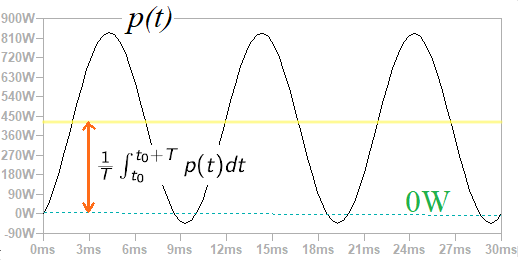
\includegraphics[width=0.4\textwidth]{src/FigAveragePower.png}
\end{center}

\end{frame}

%%%%%%%%%%%%%%%%%%%%%%%%%%%%%%%%%%%


\begin{frame}[fragile]
\frametitle{Average Power (II)}

\begin{itemize}
\item From $p(t) = \frac{V_m I_m}{2} \cos(\theta_V - \theta_I) + \frac{V_m I_m}{2} \cos(2 \omega t + \theta_V + \theta_I)$
\item Thus, average power
\\
$P = \frac{1}{T}\int_{t_0}^{t_0+T} \left\{ \frac{V_m I_m}{2} \cos(\theta_V - \theta_I) + \frac{V_m I_m}{2} \cos(2 \omega t + \theta_V + \theta_I) \right\} dt$.
\item Since integration over a period of a periodic function is $0$.
\\
$\int_{t_0}^{t_0+T} f(t) dt = 0$
when $T$ is a period of $f(t)$,
\item then
\\
$P = \frac{V_m I_m}{2} \cos(\theta_V - \theta_I) + 0$.
\end{itemize}

That is,
\begin{eqnarray}
P = \frac{V_m I_m}{2} \cos(\theta_V - \theta_I)
\label{eq: average power}.
\end{eqnarray}


\end{frame}

%%%%%%%%%%%%%%%%%%%%%%%%%%%%%%%%%%%

\begin{frame}[fragile]
\frametitle{Average Power (III)}

\begin{itemize}
\item Average power over R: $P_R = \frac{V_m I_m}{2}$
\item Average power over (ideal) L: $P_L = 0$
\item Average power over (ideal) C: $P_C = 0$
\item Average power over an impedance $\mathbb{Z} = Z_m \angle \theta_z$: $P_Z =  \frac{V_m I_m}{2} \cos \theta_z$
\\ Recall: $\mathbb{Z} = \mathbb{V}/\mathbb{I}$ and $\theta_Z = \theta_V - \theta_I$.

\end{itemize}

\end{frame}

%%%%%%%%%%%%%%%%%%%%%%%%%%%%%%%%%%%

\begin{frame}[fragile]
\frametitle{Example: Average Power (I)}

\begin{center}
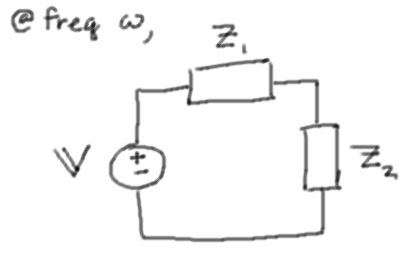
\includegraphics[width=0.4\textwidth]{src/APexample1.png}
\end{center}

\begin{itemize}
\item Find an average power over a combination of loads $Z_1$ and $Z_2$.
\item (1) Let voltage source: 20 Vp sine 100 Hz;
\\ 
$Z_1$ is a 500$\Omega$ resistor and $Z_2$ is a 200mH inductor.
\item (2) Let voltage source: 10 Vpp cosine 10 Hz;
$Z_1$ is a 1k$\Omega$ resistor and $Z_2$ is a 16$\mu$F inductor.
\end{itemize}

\end{frame}

%%%%%%%%%%%%%%%%%%%%%%%%%%%%%%%%%%%

\begin{frame}[fragile]
\frametitle{Example: Average Power (II)}

\begin{columns}[c]


\column{0.475\textwidth}
\includegraphics[width=\textwidth]{src/APexample1soln1.png}

$\mathbb{I} = \mathbb{V}/(\mathbb{Z}_1 + \mathbb{Z}_2)= 0.0388 \angle -1.817$.
$P = \frac{(20)(0.0388)}{2} \cos(-\frac{\pi}{2} + 1.817)$
\\ $\therefore P = 0.3763$ W.


\column{0.475\textwidth}
\includegraphics[width=\textwidth]{src/APexample1soln2.png}

$\mathbb{I} = 3.54m \angle 0.783$.
$P = \frac{(5)(3.54m)}{2} \cos(0-0.783)$
\\ $\therefore P = 6.59$ mW.


\end{columns}

\end{frame}

%%%%%%%%%%%%%%%%%%%%%%%%%%%%%%%%%%%

\section{RMS}

\begin{frame}[fragile]
\frametitle{Effective Values (I)}

\begin{itemize}
\item An AC voltage can be described in many ways: peak value $V_p$, peak-to-peak value $V_{pp}$, magnitude $V_m = V_p$, or amplitude $V_a = V_m = V_p$.
\item How are these quantities compared to a DC voltage?
\\
$\Rightarrow$ Rationale is to describe a magnitude of an AC voltage in a way to comprehend its real work.
\item I.e., describing the magnitude of an AC voltage by an amount of a DC voltage that will deliver the same average power to a resistor.
\end{itemize}

\end{frame}

%%%%%%%%%%%%%%%%%%%%%%%%%%%%%%%%%%%

\begin{frame}[fragile]
\frametitle{Effective Values (II)}

\vspace{-1cm}

%plot(xs, sin(xs), type='l', lwd=16, col=4)
%lines(c(0, 4*pi), c(0, 0), lty=8, col=2, lwd=4)
%lines(c(0, 4*pi), c(-0.5, -0.50), lty=8, col=5, lwd=4)
%
%plot(c(0, 4*pi), c(0.707, 0.707), col=2, lwd=16, type='l', ylim=c(-1,1))
%lines(c(0, 4*pi), c(0, 0), lty=8, col=5, lwd=8)
%
\begin{center}
\includegraphics[width=0.5\textwidth]{src/effective.png}
\end{center}

\vspace{-0.5cm}

\begin{itemize}
\item $V_{eff}$: an amount of a dc voltage that delivers the same average power as its counterpart $V_s$.
\item Average power on R by an AC voltage
\\
$P_{ac} = \frac{1}{T} \int_0^T \frac{v_s^2}{R} dt$
\item Average power on R by a DC voltage
\\
$P_{eff} = \frac{v_{eff}^2}{R}$.
\end{itemize}

\end{frame}

%%%%%%%%%%%%%%%%%%%%%%%%%%%%%%%%%%%

\begin{frame}[fragile]
\frametitle{Effective Values (III)}

\begin{center}
\includegraphics[width=0.5\textwidth]{src/effective.png}
\end{center}

Solve for $v_{eff}$ (delivering the same power as $v_s$:
%
\begin{eqnarray}
v_{eff} = \sqrt{\frac{1}{T} \int_0^T v_s^2 dt}
\label{eq: rms}.
\end{eqnarray}

\begin{itemize}
\item Since the result is obtained by squaring, averaging, and finding a square root, it is called a ``Root-Mean-Square'' value or ``RMS'' for short.
\end{itemize}

\end{frame}

%%%%%%%%%%%%%%%%%%%%%%%%%%%%%%%%%%%

\begin{frame}[fragile]
\frametitle{Effective Values (IV)}

\begin{itemize}
\item The \emph{effective value} of an ac voltage is the amount of its dc equivalence, i.e., supplying the same average power on a resistor.
\item So is an effective value of an ac current.
\end{itemize}

\begin{center}
\begin{tabular}{|c|c|}
\hline
$v_{rms} = \sqrt{\frac{1}{T} \int_0^T v_s^2 dt}$
&
$i_{rms} = \sqrt{\frac{1}{T} \int_0^T i_s^2 dt}$
\\ \hline
\end{tabular}
\end{center}

\begin{center}
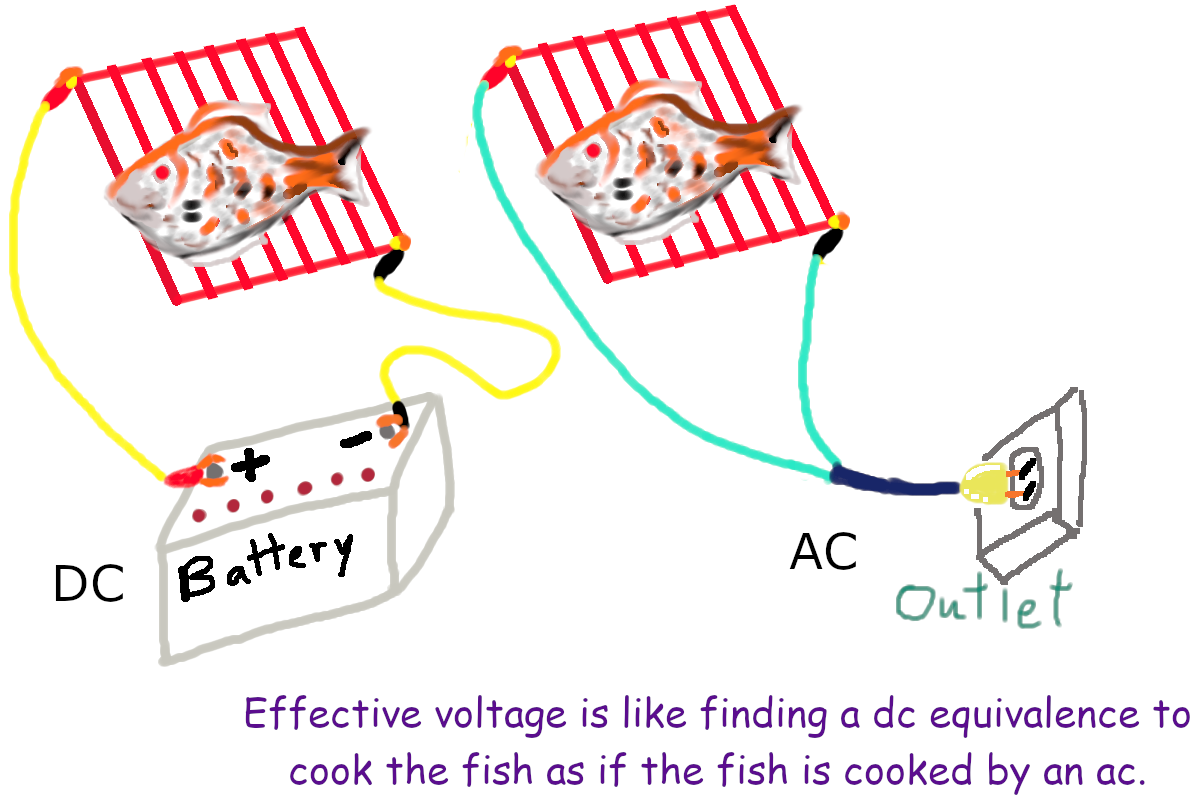
\includegraphics[width=0.5\textwidth]{src/rmsFish.png}
\end{center}

\end{frame}

%%%%%%%%%%%%%%%%%%%%%%%%%%%%%%%%%%%

\begin{frame}[fragile]
\frametitle{RMS on Sinusoid}

\vspace{-0.2cm}

Given $v_s(t) = V_m \cos(\omega t)$,
%
\vspace{-0.2cm}
%
\begin{eqnarray}
V_{rms} &=& \sqrt{\frac{1}{T} \int_0^T \left( V_m \cos(\omega t)\right)^2 dt}
\nonumber \\
&=& V_m \sqrt{\frac{1}{T} \int_0^T \cos^2(\omega t) dt}
\nonumber \\
&=& V_m \sqrt{\frac{1}{T} \int_0^T \frac{1 + \cos(2 \omega t)}{2} dt}
\nonumber \\
&=& V_m \sqrt{\frac{1}{2} \cdot \underbrace{\frac{1}{T} \int_0^T 1 dt}_1 + \underbrace{\frac{1}{T}\int_0^T  \frac{\cos(2 \omega t)}{2} dt}_0 }
\nonumber \\
&=& \frac{V_m}{\sqrt{2}}
\label{eq: Vrms}.
\end{eqnarray}

\end{frame}

%%%%%%%%%%%%%%%%%%%%%%%%%%%%%%%%%%%

\begin{frame}[fragile]
\frametitle{RMS Values}

\begin{itemize}
\item $V_{rms} = \frac{V_m}{\sqrt{2}}$
\item $I_{rms} = \frac{I_m}{\sqrt{2}}$
\end{itemize}

\vspace{1cm}

$\Rightarrow$ Conveniently, average power
\begin{eqnarray}
P &=& \frac{V_m \cdot I_m}{2} \cos(\theta_V - \theta_I)
\nonumber \\
&=& \frac{V_m}{\sqrt{2}} \cdot \frac{I_m}{\sqrt{2}} \cos(\theta_V - \theta_I)
\nonumber \\
&=& V_{rms}  \cdot I_{rms} \cos(\theta_V - \theta_I)
\nonumber .
\end{eqnarray}


\end{frame}

%%%%%%%%%%%%%%%%%%%%%%%%%%%%%%%%%%%

\section{Complex power}

\begin{frame}[fragile]
\frametitle{Complex Power (I)}

\begin{center}
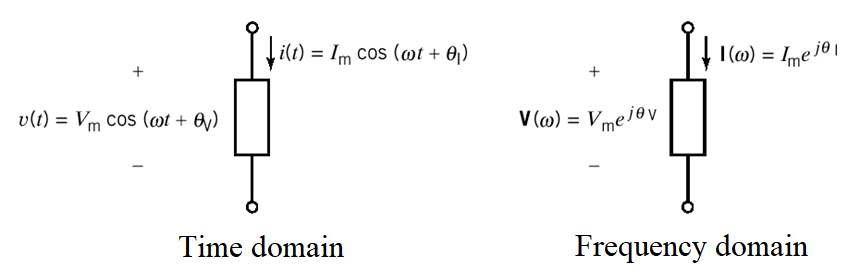
\includegraphics[width=0.9\textwidth]{src/ComplexPower.png}
\end{center}

\begin{itemize}
\item voltage and current can be represented in frequency domain as complex numbers.
\item So is power!
\end{itemize}

\end{frame}

%%%%%%%%%%%%%%%%%%%%%%%%%%%%%%%%%%%

\begin{frame}[fragile]
\frametitle{Complex Power (I)}

Given $\mathbb{V} = V_m \angle \theta_V$
and $\mathbb{I} = I_m \angle \theta_I$,
complex power delivered to the element is defined as:
%
\begin{eqnarray}
\mathbb{S} = \frac{\mathbb{V} \cdot \mathbb{I}^\ast}{2}
&=& \frac{(V_m \angle \theta_V) \cdot (I_m \angle -\theta_I)}{2}
\nonumber \\
&=& \frac{V_m \cdot I_m}{2} \angle (\theta_V -\theta_I)
\nonumber \\
&=& V_{rms} \cdot I_{rms} \angle (\theta_V -\theta_I)
\label{eq: complex power}
\end{eqnarray}
where $\mathbb{I}^\ast$ is a complex conjugate of $\mathbb{I}$.

\end{frame}

%%%%%%%%%%%%%%%%%%%%%%%%%%%%%%%%%%%

\begin{frame}[fragile]
\frametitle{Complex Power (II)}

\begin{itemize}
\item Complex power $\mathbb{S} = \frac{V_m \cdot I_m}{2} \angle (\theta_V -\theta_I)$.
\item Magnitude $|\mathbb{S}| = \frac{V_m \cdot I_m}{2}$ is called ``apparent power''.
\item Its rectangular form:
\\
$\mathbb{S} = \underbrace{\frac{V_m \cdot I_m}{2} \cos(\theta_V - \theta_I)}_P + j \underbrace{\frac{V_m \cdot I_m}{2} \sin(\theta_V - \theta_I)}_Q$
\\
$\mathbb{S} = P +jQ$.
\item Its real part $P$ is average power or real power.
\item Its imaginary part $Q$ is called ``reactive power''.
\item $\mathbb{S}$'unit is VA (Volt-Amp).
\\
$P$'s is W.
\\
$Q$'s is VAR (Volt-Amp Reactive).
\end{itemize}

\end{frame}

%%%%%%%%%%%%%%%%%%%%%%%%%%%%%%%%%%%

\section{Power factor}

\begin{frame}[fragile]
\frametitle{Power Factor}

\begin{itemize}
\item Complex power $\mathbb{S} = \underbrace{\frac{V_m \cdot I_m}{2} \cos(\theta_V - \theta_I)}_P + j \underbrace{\frac{V_m \cdot I_m}{2} \sin(\theta_V - \theta_I)}_Q$.
\item Real power $P =   \underbrace{\frac{V_m \cdot I_m}{2}}_{|\mathbb{S}|} \cdot \underbrace{\cos(\theta_V - \theta_I)}_{\mbox{power factor}}$.
\item Power factor $pf = \cos(\theta_V - \theta_I)$.
\item pf angle $\theta_V - \theta_I > 0$ $\Rightarrow$ ``lagging''
\\
Current lags voltage $\rightarrow$ inductive load.
%
\item pf angle $\theta_V - \theta_I = 0$ $\Rightarrow$ ``in-phase''
\\
Current and voltage are in-phase $\rightarrow$ purely resistive load.
%
\item pf angle $\theta_V - \theta_I < 0$ $\Rightarrow$ ``leading''
\\
Current leads voltage $\rightarrow$ capacitive load.
\end{itemize}

\end{frame}

%%%%%%%%%%%%%%%%%%%%%%%%%%%%%%%%%%%


\begin{frame}[fragile]
\frametitle{Example: Load Impedance (I)}

An electric load operates at 240 Vrms. The load consumes an average power of 8 kW at a lagging power factor of 0.8.
\\
(a) Calculate the complex power of the load.
\\
(b) Calculate the impedance of the load.
\\

Solution for (a):
\begin{itemize}
\item $pf = \cos(\phi) = 0.8$ and
$P = 8kW = |\mathbb{S}| \cdot \cos(\phi)$.
\\
$\Rightarrow |\mathbb{S}| = 8k/0.8 = 10$ kVA.
\item lagging $\Rightarrow$ $\phi > 0$.
\\
$\Rightarrow \phi = \cos^{-1} 0.8 = 0.6435$ rad.
\item $\therefore Q = |\mathbb{S}| \cdot \sin(\phi) = 10k \sin(0.6435) = 6$ kVAR.
\item $\mathbb{S} = P + jQ = 8 + j6$ kVA. 
\end{itemize}

\end{frame}


%%%%%%%%%%%%%%%%%%%%%%%%%%%%%%%%%%%


\begin{frame}[fragile]
\frametitle{Example: Load Impedance (II)}

\begin{center}
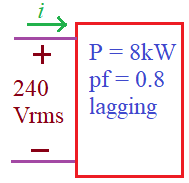
\includegraphics[width=0.2\textwidth]{src/pf_impedance.png}
\end{center}


Solution for (b):
\begin{itemize}
\item $P = 8kW = \frac{V_m I_m}{2} \cdot pf$
$= V_{rms} \cdot I_{rms} \cdot pf$
$= 240 \cdot I_{rms} \cdot 0.8$
\\ $\Rightarrow I_{rms} = 41.67$ A.
\item Impedance $\mathbb{Z} = \frac{\mathbb{V}}{\mathbb{I}}$
$= \frac{V_m}{I_m} \angle (\theta_V - \theta_I)$
$= \frac{V_{rms}}{I_{rms}} \angle \phi$
$= \frac{240}{41.67} \angle 0.6435$.
\\
$\Rightarrow \mathbb{Z} =  4.608 + j3.456$ $\Omega$.

\end{itemize}

\end{frame}

%%%%%%%%%%%%%%%%%%%%%%%%%%%%%%%%%%%

\begin{frame}[fragile]
\frametitle{PF and Transmission Loss (I)}

The transmission lines for electrical power

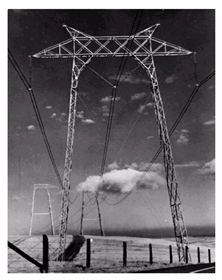
\includegraphics[height=1.5in]{src/TransmissionLines.png}
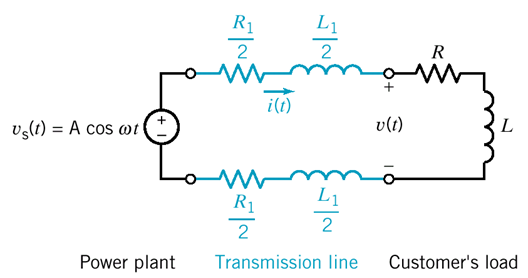
\includegraphics[height=1.5in]{src/TransmissionLinesCCT.png}


%\begin{columns}[c]
%\column{0.2\textwidth}
%
%\column{0.75\textwidth}
%
\begin{itemize}
\item Transmission lines are significantly different from ideal wires.
\\ $\mathbb{Z}_{line} = R_1 + j \omega L_1$.
\item Average power losing on the lines
\\ $P_{line} = I_{rms}^2 \cdot Re\{ \mathbb{Z}_{line} \}$
$=I_{rms}^2 R_1$.
\end{itemize}
%\end{columns}

\end{frame}

%%%%%%%%%%%%%%%%%%%%%%%%%%%%%%%%%%%

\begin{frame}[fragile]
\frametitle{PF and Transmission Loss (II)}

\begin{columns}[c]
\column{0.3\textwidth}
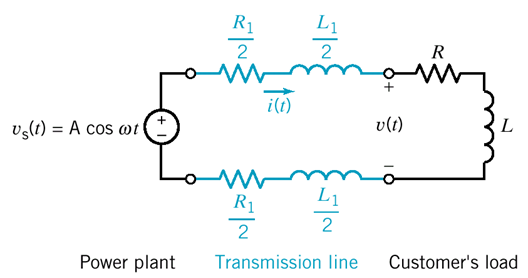
\includegraphics[width=\textwidth]{src/TransmissionLinesCCT.png}

\column{0.65\textwidth}
Average power losing on the lines
\\ $P_{line} = I_{rms}^2 \cdot Re\{ \mathbb{Z}_{line} \}$
$=I_{rms}^2 R_1$.
\end{columns}

\begin{itemize}
\item A large load is often inductive, e.g., machine, motor, pump, etc.
\item Power consumed by the load is what its owner pays.
\\
$P_{load} = V_{rms} I_{rms} \cdot pf$.
\item Power losing on the lines is just a waste of energy, which customers do not pay, but it costs an electric supplier.
\item Given the same $P_{load}$ and operating voltage $V_{rms}$,
a lower $pf$ causes a higher current $I_{rms}$.
And, a higher current $I_{rms}$ $\Rightarrow$ a higher $P_{line}$.
\end{itemize}


\end{frame}

%%%%%%%%%%%%%%%%%%%%%%%%%%%%%%%%%%%

\begin{frame}[fragile]
\frametitle{PF and Transmission Loss (III)}

\begin{columns}[c]
\column{0.3\textwidth}
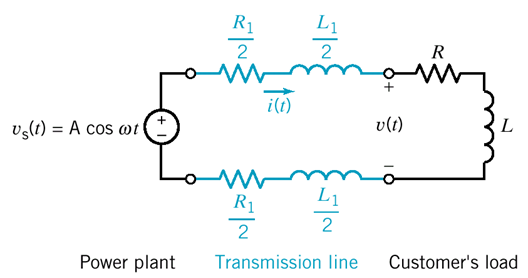
\includegraphics[width=\textwidth]{src/TransmissionLinesCCT.png}

\column{0.65\textwidth}
$P_{load} = V_{rms} I_{rms} \cdot pf$.
\\
$P_{line} = I_{rms}^2 \cdot Re\{ \mathbb{Z}_{line} \}$
$=I_{rms}^2 R_1$.

\end{columns}
\vspace{0.5cm}

Example: a 1.4kW Load with a lagging power factor of 0.8, operated at 220 Vrms 50Hz.

\begin{itemize}
\item Current $i$ drawn by the load: $I_{rms} = \frac{1.4k}{(220)(0.8)}$ $=7.95$ A.
\item Supposed $R_1 = 1$ $\Omega$, $P_{line} = (7.95)^2 (1) = 63.27$ W.
%\\
%$\Rightarrow$ That's 4.5\% loss! ($\frac{63.25}{1.4k} \cdot 100 = 4.5$)
\\
$\Rightarrow$
{\small
To put it in perspective, if the load is run 20 hr/day, 350 days a year,
that counts 7000 hours.
Supposed the price is 5 baht/unit, energy loss: $E_{loss} = (63.27)(7000) = 442890$ Wh $=442.89$ units.
\\ Thus, estimated loss is 2214.45 baht for this one customer. 
%(Now, Imagine 180 new factories opening each month!)
}%small
\end{itemize}

\end{frame}

%%%%%%%%%%%%%%%%%%%%%%%%%%%%%%%%%%%


\begin{frame}[fragile]
\frametitle{PF and Transmission Loss (III)}

\begin{columns}[c]
\column{0.3\textwidth}
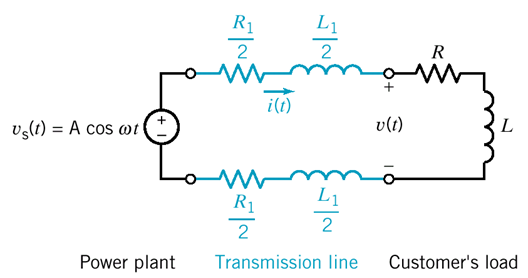
\includegraphics[width=\textwidth]{src/TransmissionLinesCCT.png}

\column{0.65\textwidth}
$I_{rms} = \frac{P_{load}}{V_{rms} \cdot pf}$.
\\
$P_{line} = I_{rms}^2 R_1$.

\end{columns}
\vspace{0.5cm}

Line loss as a function of power factor

\begin{columns}[c]
\column{0.3\textwidth}
\begin{eqnarray}
P_{line} = \left( \frac{P_{load}}{V_{rms} \cdot pf} \right)^2 R_1
\nonumber .
\end{eqnarray}

\column{0.6\textwidth}
%Pline = function(pf){ 100*(1/pf)^2 }
%f = seq(0.8, 1, 1e-2)
%plot(f, Pline(f)-100, type='l', xlab='pf', ylab='%Extra loss', main='Line loss by power factor')
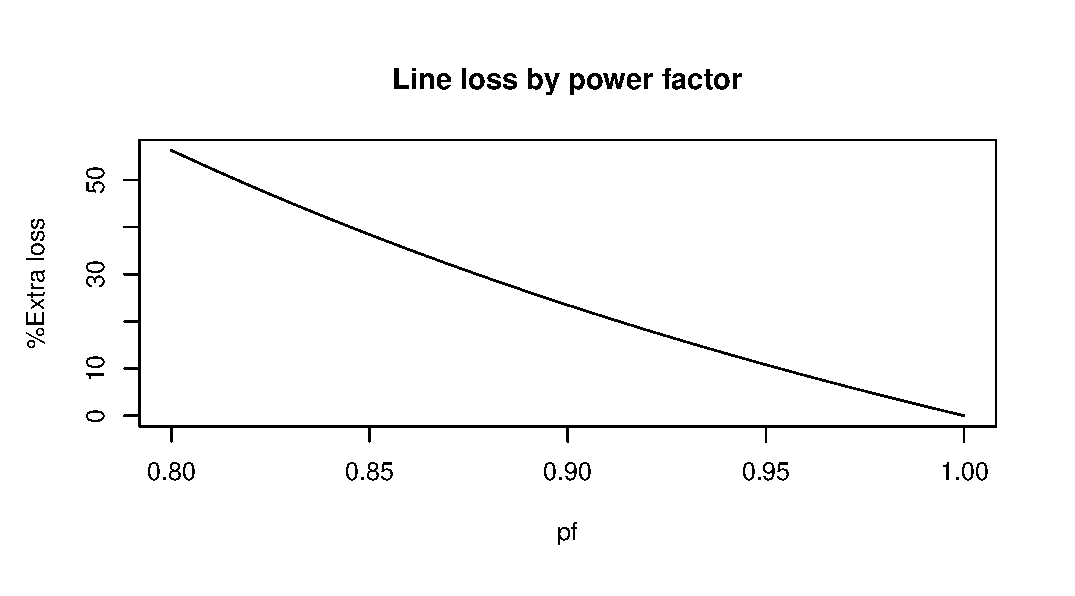
\includegraphics[width=\textwidth]{src/Pline_pf.eps}
\end{columns}

With pf of 0.8, the power line loss is over 50\% of the ideal case ($pf = 1$).





\end{frame}

%%%%%%%%%%%%%%%%%%%%%%%%%%%%%%%%%%%

\begin{frame}[fragile]
\frametitle{Power Factor Correction (I)}

\begin{center}
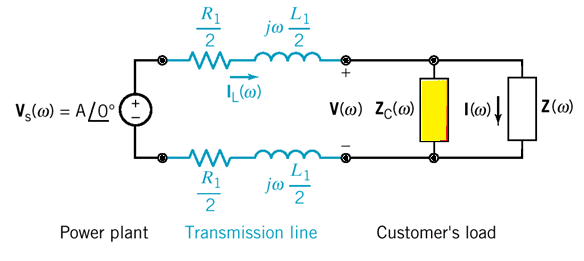
\includegraphics[width=0.5\textwidth]{src/pfc0.png}
\end{center}

\begin{itemize}
\item To mitigate, a customer is required to have the power factor above an agreeable level.
\item To ``correct'' power factor of a load, a correcting impedance is installed across the terminals of the customer's load.
\\
$\Rightarrow$ having the correcting impedance parallel to the load retains the load operating voltage.

\end{itemize}

\end{frame}

%%%%%%%%%%%%%%%%%%%%%%%%%%%%%%%%%%%

\begin{frame}[fragile]
\frametitle{Power Factor Correction (II)}

\vspace{-0.5cm}
\begin{center}
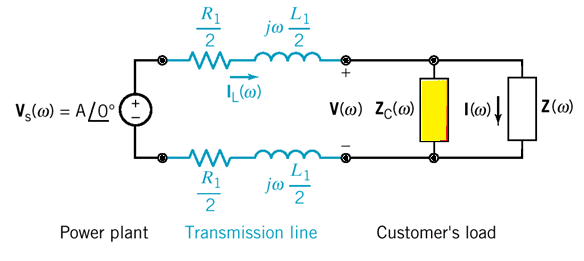
\includegraphics[width=0.5\textwidth]{src/pfc0.png}
\end{center}
\vspace{-0.5cm}

The correcting impedance should turn power factor of the load to
%
%\vspace{-0.5cm}
\begin{align*}
pfc = \cos \phi_p
\nonumber ,
\end{align*}
%\vspace{-1cm}
%
where $pfc$ and $\phi_p$ are the target power factor and  the target pf angle.

{\small
$\quad$ Given load impedance $\mathbb{Z} = R + jX$ and correcting impedance $\mathbb{Z}_c = R_c + jX_c$, the correcting impedance should not consume power itself: 
$R_c = 0$ $\Rightarrow$ 
$\mathbb{Z}_c = jX_c$.
(It must be purely reactive, C or L.)
}%small

\end{frame}

%%%%%%%%%%%%%%%%%%%%%%%%%%%%%%%%%%%

\begin{frame}[fragile]
\frametitle{Power Factor Correction (III)}

\vspace{-1cm}
\begin{columns}[c]
\column{0.475\textwidth}
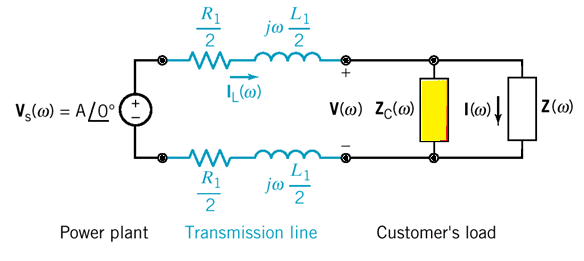
\includegraphics[width=\textwidth]{src/pfc0.png}

\column{0.475\textwidth}
Target power factor: $pfc = \cos \phi_p$.
\\
Original load: $\mathbb{Z} = R + jX$.
Correcting impedance: $\mathbb{Z}_c = jX_c$.
\end{columns}

\begin{itemize}
\item corrected impedance: $\mathbb{Z}_p = \frac{\mathbb{Z} \mathbb{Z}_c}{\mathbb{Z} + \mathbb{Z}_c}$
$= R_p +jX_p$
$=Z_p \angle \theta_p$.
\item note: pf angle = load angle, i.e., $\theta_p = \phi_p$.
\\
$\Rightarrow$
$\mathbb{Z}_p = Z_p \angle \phi_p$
\\
$\Rightarrow$ $\phi_p = \tan^{-1} \frac{X_p}{R_p}$
$\Rightarrow$
$pfc = \cos( \tan^{-1} \frac{X_p}{R_p} )$
$\Rightarrow$
$\frac{X_p}{R_p} = \tan ( \cos^{-1} pfc )$.
\end{itemize}

\end{frame}

%%%%%%%%%%%%%%%%%%%%%%%%%%%%%%%%%%%

\begin{frame}[fragile]
\frametitle{Power Factor Correction (IV)}

{\color{blue}\small
%\vspace{-1cm}
\begin{columns}[c]
\column{0.4\textwidth}
(1) $\mathbb{Z}_p = \frac{\mathbb{Z} \mathbb{Z}_c}{\mathbb{Z} + \mathbb{Z}_c}$
$= R_p +jX_p$.
\\
(2) $\frac{X_p}{R_p} = \tan ( \cos^{-1} pfc )$.

\column{0.55\textwidth}
Target: $pfc = \cos \phi_p$.
\\
Impedances: $\mathbb{Z} = R + jX$
and $\mathbb{Z}_c = jX_c$.
\end{columns}
}%
\vspace{0.5cm}

Work the math, from (1):
\begin{eqnarray}
\mathbb{Z}_p &=& \frac{(R + jX) (jX_c)}{(R + jX) + jX_c}
= \underbrace{\frac{R X_c^2}{R^2 + (X + X_c)^2}}_{R_p} + j \underbrace{\frac{R^2 X_c + (X_c + X) X X_c}{R^2 + (X + X_c)^2}}_{X_p}
\nonumber .
\end{eqnarray}
Put the result into (2):
\begin{eqnarray}
\frac{R^2 X_c + (X_c + X) X X_c}{R X_c^2} = \tan ( \cos^{-1} pfc )
\nonumber .
\end{eqnarray}

\end{frame}

%%%%%%%%%%%%%%%%%%%%%%%%%%%%%%%%%%%


\begin{frame}[fragile]
\frametitle{Power Factor Correction (V)}

\begin{center}
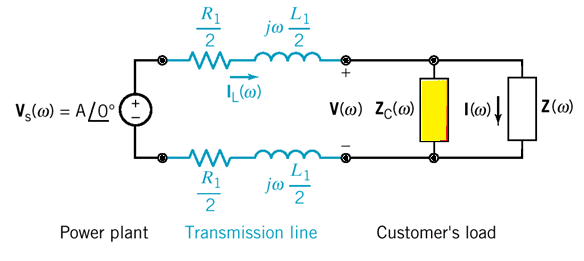
\includegraphics[width=0.5\textwidth]{src/pfc0.png}
\end{center}

Solve for $X_c$ in terms of $R$, $X$, and $pfc$:
\begin{eqnarray}
X_c = \frac{R^2 + X^2}{R \tan(\cos^{-1} pfc) - X}
\label{eq: pf correction}.
\end{eqnarray}

\end{frame}

%%%%%%%%%%%%%%%%%%%%%%%%%%%%%%%%%%%


\begin{frame}[fragile]
\frametitle{Example: Power Factor Correction}

\vspace{-0.5cm}

\begin{columns}[c]
\column{0.48\textwidth}
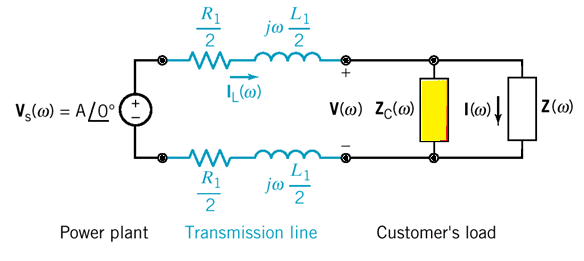
\includegraphics[width=\textwidth]{src/pfc0.png}
%
\column{0.48\textwidth}
Reactive value:
$X_c = \frac{R^2 + X^2}{R \tan(\cos^{-1} pfc) - X}$
\end{columns}

Example. 
A 1.4kW load with a lagging pf of 0.8, operating at 220 Vrms 50 Hz,
is required to be corrected for pf of 0.95.
\\
\underline{Solution:} \\
Recalling from the previous example,
$I_{rms} = 7.95$ A.
Then, $\mathbb{Z} = \frac{220}{7.95} \angle (\underbrace{+}_{lagging}\cos^{-1} 0.8)$
$= 27.67 \angle 0.64$
$= 22.19 + j16.52$ $\Omega$.

Thus, $X_c = \frac{22.19^2 + 16.52^2}{22.19 \cdot \tan(\cos^{-1} 0.95) - 16.52}$ 
$= -82.9$.
Since $X_c < 0$, the correcting impedance must be capacitive:
$X_c = -\frac{1}{\omega C}$. Given $\omega = 2\pi(50) = 314.16$ rad/s, $C = 38.4$ $\mu$F (or larger).

\end{frame}
% Double check
% Z = 22.19 + 16.52i
% cos(Arg(Z)) % Original pf
%[1] 0.8021205
% Zc = 1/(1i*314.16*38.4e-6)
% Zp = 1/(1/Z + 1/Zc)
% cos(Arg(Zp)) % pfc
% [1] 0.9500757

%%%%%%%%%%%%%%%%%%%%%%%%%%%%%%%%%%%

\begin{frame}[fragile]
\frametitle{Power Factor Correction: Inductive Load (I)}

\vspace{-0.5cm}

\begin{columns}[c]
\column{0.48\textwidth}
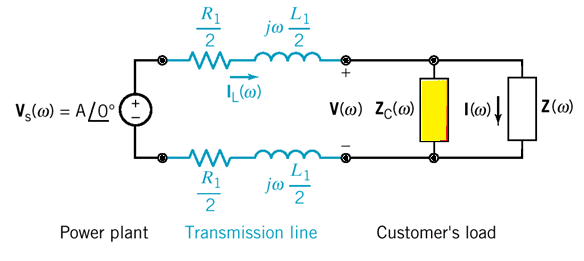
\includegraphics[width=\textwidth]{src/pfc0.png}
%
\column{0.48\textwidth}
Reactive value:
$X_c = \frac{R^2 + X^2}{R \tan(\cos^{-1} pfc) - X}$
\end{columns}

\begin{itemize}
\item The larger $pfc$ (closer to 1), the better.
\item $pfc \rightarrow 1$ 
$\Rightarrow \cos^{-1} pfc \rightarrow 0$ 
$\Rightarrow \tan(\cos^{-1} pfc) \rightarrow 0$.
\item Sign of $X_c$ is opposite to the sign of $X$.
\\
$\Rightarrow$ Correct capacitive load with inductor. 
\\
$\Rightarrow$ Correct inductive load with capacitor.
\end{itemize}

\end{frame}

%%%%%%%%%%%%%%%%%%%%%%%%%%%%%%%%%%%

\begin{frame}[fragile]
\frametitle{Power Factor Correction: Inductive Load (II)}

%\vspace{-0.5cm}
%
%\begin{columns}[c]
%\column{0.48\textwidth}
%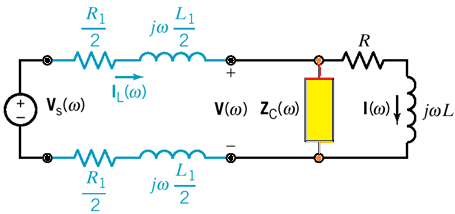
\includegraphics[width=\textwidth]{src/pfc.png}
%%
%\column{0.48\textwidth}
%(1)
%$X_c = \frac{R^2 + X^2}{R \tan(\cos^{-1} pfc) - X}$
%\end{columns}

Typical loads are inductive. Thus, $X_c = -\frac{1}{\omega C}$
and
%Put (2) into (1),
\begin{eqnarray}
-\frac{1}{\omega C} &=& \frac{R^2 + X^2}{R \tan(\cos^{-1} pfc) - X}
\nonumber \\
\omega C &=& \frac{X - R \tan(\cos^{-1} pfc)}{R^2 + X^2}
\nonumber \\
&=& \frac{R}{R^2 + X^2} \cdot \left( \frac{X}{R} - \tan(\cos^{-1} pfc) \right)
\nonumber .
\end{eqnarray}

Given an original pf angle $\phi = \tan^{-1} \frac{X}{R}$, 
hence 
\begin{eqnarray}
C = \frac{R}{\omega \cdot (R^2 + X^2)} \cdot \left( \tan \phi - \tan \phi_c \right)
\label{eq: pfc C},
\end{eqnarray}
where $\phi = \cos^{-1} pf$ and $\phi_c = \cos^{-1} pfc$.

\end{frame}

%%%%%%%%%%%%%%%%%%%%%%%%%%%%%%%%%%%

\begin{frame}[fragile]
\frametitle{Example: Power Factor Correction on Inductive Load}

\vspace{-0.5cm}

\begin{columns}[c]
\column{0.4\textwidth}
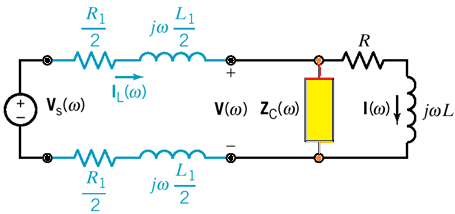
\includegraphics[width=\textwidth]{src/pfc.png}
%
\column{0.56\textwidth}
Given the original load $\mathbb{Z} = 100 + j100$ $\Omega$
at 60 Hz, find C to improve pf to 0.95.

\end{columns}
\underline{Solution}:
\begin{itemize}
\item $\phi = \tan^{-1} \frac{X}{R}$ 
$= 0.785$ rad.
\item $\phi_c = \cos^{-1} pfc$
$= 0.318$ rad.
\item $\omega = 2\pi f$
$= 377$ rad/s.
\item $C = \frac{100}{377 \cdot (100^2 + 100^2)} \cdot \left( \tan 0.785 - \tan 0.318 \right)$
$=8.9$ $\mu$F (or larger).
\end{itemize}

\end{frame}

%%%%%%%%%%%%%%%%%%%%%%%%%%%%%%%%%%%

\section{Power superposition}

\begin{frame}[fragile]
\frametitle{Power Superposition for Multi-Frequency Excitation (I)}

\begin{center}
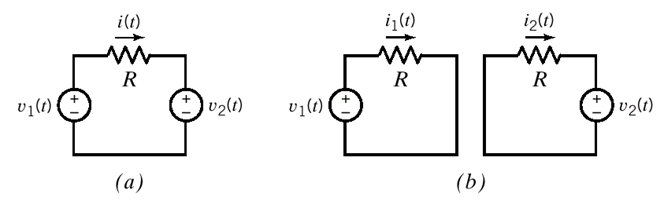
\includegraphics[width=0.6\textwidth]{src/super1.png}
\end{center}

\begin{itemize}
\item Superposition: $i = i_1 + i_2$.
\item Instantaneous power: $p = i^2 R = (i_1 + i_2)^2 R$
$=(i_1^2 + i_2^2 + 2 i_1 i_2) R$.
\end{itemize}

Average power: 
\begin{eqnarray}
P &=& \frac{1}{T} \int_{0}^T p(t) dt = \frac{1}{T} \int_{0}^T (i_1^2 + i_2^2 + 2 i_1 i_2) R dt
\nonumber \\
&=& P_1 + P_2 + \frac{2 R}{T} \int_{0}^T (i_1 \cdot i_2) dt
\nonumber .
\end{eqnarray}

\emph{Caution!} Superposition principle cannot apply to power in 
\end{frame}

%%%%%%%%%%%%%%%%%%%%%%%%%%%%%%%%%%%

\begin{frame}[fragile]
\frametitle{Power Superposition for Multi-Frequency Excitation (II)}

\begin{columns}[c]

\column{0.475\textwidth}
\includegraphics[width=\textwidth]{src/super1.png}

\column{0.475\textwidth}
Average power: 
$P = P_1 + P_2 + \frac{2 R}{T} \underbrace{\int_{0}^T (i_1 \cdot i_2) dt}$

\end{columns}

Given $i_1 = I_1 \cos(\omega_1 t + \theta_1)$
and $i_2 = I_2 \cos(\omega_2 t + \theta_2)$,
%\begin{eqnarray}
$\int_{0}^T (i_1 \cdot i_2) dt
= I_1 I_2 \int_{0}^T \cos(\omega_1 t + \theta_1) \cos(\omega_2 t + \theta_2) dt$.
\\
%\nonumber .
%\end{eqnarray}

\vspace{0.5cm}
From $\cos A \cos B = \frac{\cos(A-B) + \cos(A+B)}{2}$,
\begin{eqnarray}
\int_{0}^T (i_1 \cdot i_2) dt
&=& \frac{I_1 I_2}{2} \int_{0}^T \left(
\cos( (\omega_1 - \omega_2) t + \theta_1 - \theta_2) 
\right) dt
\nonumber \\
&\;&
+
\frac{I_1 I_2}{2} \underbrace{\int_{0}^T \left(
+ \cos( (\omega_1 + \omega_2) t + \theta_1 + \theta_2) 
\right) dt}_{0}
\nonumber .
\end{eqnarray}

\end{frame}

%%%%%%%%%%%%%%%%%%%%%%%%%%%%%%%%%%%

\begin{frame}[fragile]
\frametitle{Power Superposition for Multi-Frequency Excitation (III)}

\begin{columns}[c]

\column{0.475\textwidth}
\includegraphics[width=\textwidth]{src/super1.png}

\column{0.475\textwidth}
Average power: 
$P = P_1 + P_2 + \frac{2 R}{T} \underbrace{\int_{0}^T (i_1 \cdot i_2) dt}$

\end{columns}

\begin{eqnarray}
\int_{0}^T (i_1 \cdot i_2) dt
&=& \frac{I_1 I_2}{2} \int_{0}^T \left(
\cos( (\omega_1 - \omega_2) t + \theta_1 - \theta_2) 
\right) dt
\nonumber \\
&=& \left\{
\begin{array}{ll}
0 & \mbox{ for } \omega_1 \neq \omega_2,
\\
\frac{I_1 I_2 T}{2} \cos(\theta_1 - \theta_2)
& \mbox{ for } \omega_1 = \omega_2.
\end{array}
\right.
\nonumber 
\end{eqnarray}
That is,
\begin{eqnarray}
P &=& P_1 + P_2 + \left\{
\begin{array}{ll}
0 & \mbox{ for } \omega_1 \neq \omega_2,
\\
I_1 I_2 R \cos(\theta_1 - \theta_2)
& \mbox{ for } \omega_1 = \omega_2.
\end{array}
\right.
\label{eq: power superposition}
\end{eqnarray}

\end{frame}

%%%%%%%%%%%%%%%%%%%%%%%%%%%%%%%%%%%

\begin{frame}[fragile]
\frametitle{Power Superposition for Multi-Frequency Excitation (III)}

``The \emph{average power} delivered to a circuit by several sinusoidal sources, acting together, is equal to the sum of the average power delivered to the circuit by each source acting alone, \emph{\color{red} if and only if no two of the sources have the same frequency.}''

\begin{eqnarray}
P_{total} &=& P_1 + P_2 + \cdots + P_N
\nonumber \\
&=& \sum_i P_i
\nonumber ,
\end{eqnarray}
where $P_i$ is a power computed as if the $i^{th}$ sinusoidal source acting alone and \underline{\color{blue}no two sources have the same frequency.}


\emph{\color{red}Caution!} Superposition principle cannot be applied to power in general.
\end{frame}

%%%%%%%%%%%%%%%%%%%%%%%%%%%%%%%%%%%

\begin{frame}[fragile]
\frametitle{Example: Power Superposition (I)}

\begin{columns}[c]

\column{0.3\textwidth}
\includegraphics[width=\textwidth]{src/super_example1.png}

\column{0.6\textwidth}
Find power $P_R$ consumed by R in this setting:
$v_A(t) = 155.6 \cos(377 t)$;
$i_B(t) = 1.2 \cos(314.16 t)$;
\\
$R = 50$ $\Omega$ and $L = 0.5$ H.
\end{columns}

\underline{Solution}:
\begin{itemize}
\item Both sources have different frequencies.
\\
$\Rightarrow$ use superposition to work on one source at a time.
\item Since both sources are sinusoidal and have different frequencies,
power superposition can be applied.
\\
$P_R = P_R(v_A) + P_R(i_B)$.
\end{itemize}


\end{frame}
%%%%%%%%%%%%%%%%%%%%%%%%%%%%%%%%%%%

\begin{frame}[fragile]
\frametitle{Example: Power Superposition (II)}

\begin{columns}[c]

\column{0.475\textwidth}
\includegraphics[width=2cm]{src/super_example1a.png}
\begin{itemize}
\item $\omega_1 = 377$ rad/s
\item $Z_R = 50$; $Z_L = j188.5$.
\item $\mathbb{V}_A = 155.6 \angle 0$.
\item $\mathbb{I}_1 =  \frac{\mathbb{V}_A}{50 + j188.5}$
$=0.798 \angle -1.31$
\item $P_R(v_A) = I_{1rms}^2 R$
$=\left(\frac{0.798}{\sqrt{2}}\right)^2 50$
$=15.92$ W.
\end{itemize}

\column{0.475\textwidth}
\includegraphics[width=2cm]{src/super_example1b.png}
\begin{itemize}
\item $\omega_2 = 314.16$ rad/s
\item $Z_R = 50$; $Z_L = j157.08$.
\item $\mathbb{I}_B = 1.2 \angle 0$.
\item $\mathbb{I}_2 =  -\mathbb{I}_B \cdot \frac{\mathbb{Y}_R}{\mathbb{Y}_R + \mathbb{Y}_L}$ 
$=-1.2 \frac{(1/50)}{(1/50) + (1/j157.08)}$
$= 1.143 \angle -2.83$.
\item $P_R(i_B) = I_{2rms}^2 R$
$=\left(\frac{1.143}{\sqrt{2}}\right)^2 50$
$=32.69$ W.
\end{itemize}

\end{columns}

%\begin{itemize}
%\item $P_R = P_R(v_A) + P_R(i_B)$.
%\end{itemize}


\end{frame}
%%%%%%%%%%%%%%%%%%%%%%%%%%%%%%%%%%%

\begin{frame}[fragile]
\frametitle{Example: Power Superposition (III)}

\begin{center}
\includegraphics[width=0.5\textwidth]{src/super_example1.png}
\end{center}

Since both sources have different frequency,
the power superposition is valid:
\begin{eqnarray}
P_R &=& P_R(v_A) + P_R(i_B)
\nonumber \\
&=& 15.92 + 32.69 = 48.61 W
\nonumber.
\end{eqnarray}


\end{frame}
%%%%%%%%%%%%%%%%%%%%%%%%%%%%%%%%%%%

\section{Maximum power transfer}

\begin{frame}[fragile]
\frametitle{Maximum Average Power Transfer (I)}

\begin{columns}[c]

\column{0.2\textwidth}
\includegraphics[width=\textwidth]{src/Max1.png}

\column{0.75\textwidth}
\begin{itemize}
\item At some situation, we may want to find a load $Z_L$ such that the power delivered to the load is maximum.
\end{itemize}

\end{columns}

\begin{columns}[c]

\column{0.7\textwidth}
\begin{itemize}
\item To simplify the task, the portal circuit is modeled by Thevenin equivalent circuit.
\end{itemize}

\column{0.25\textwidth}
\includegraphics[width=\textwidth]{src/Max2.png}

\end{columns}

\begin{itemize}
\item Supposed $\mathbb{Z}_{Th} = R_{Th} + jX_{Th}$
and $\mathbb{Z}_L = R_L + jX_L$,
current $\mathbb{I} = \frac{\mathbb{V}_{Th}}{\mathbb{Z}_{Th} + \mathbb{Z}_L}$.
\item Average power $P_R = \frac{V_m I_m}{2} = \frac{1}{2} I_m^2 R_L$
$=\frac{1}{2} \frac{ |\mathbb{V}_{Th}|^2 R_L}{(R_{Th} + R_L)^2 + (X_{Th} + X_L)^2}$
\item Find $X_L$ and $R_L$ maximizing $P_R$.
\end{itemize}

\end{frame}
%%%%%%%%%%%%%%%%%%%%%%%%%%%%%%%%%%%

\begin{frame}[fragile]
\frametitle{Maximum Average Power Transfer (II)}

\begin{tabular}{ccl}
\includegraphics[height=1.8cm]{src/Max1.png}
&
\includegraphics[height=2cm]{src/Max2.png}
&
$P_R = \frac{1}{2} \frac{ |\mathbb{V}_{Th}|^2 R_L}{(R_{Th} + R_L)^2 + (X_{Th} + X_L)^2}$.
\end{tabular}

\begin{itemize}
\item Notice that $X_L = - X_{Th}$ maximizing $P_R$.
\item Solve $\frac{\partial P_R}{\partial R_L} = 0$ for $R_L$
\\
$\Rightarrow$ $R_L = R_{Th}$.
\end{itemize}

Thus,
\begin{equation}
\mathbb{Z}_L = R_{Th} - jX_{Th} = \mathbb{Z}^\ast_{Th}
\label{eq: Z max power transfer}.
\end{equation}

The maximum power is:
\begin{equation}
P_{\max} = \frac{|\mathbb{V}_{Th}|_{Th}^2}{8 R_{Th}}
\label{eq: max power transfer}.
\end{equation}

\end{frame}
%%%%%%%%%%%%%%%%%%%%%%%%%%%%%%%%%%%

\begin{frame}[fragile]
\frametitle{Example: Maximum Average Power Transfer (I)}

\begin{columns}[c]

\column{0.62\textwidth}
Determine the load impedance $\mathbb{Z}_L$ maximizing the average power drawn from the circuit.
What is the maximum average power?

\column{0.35\textwidth}
\includegraphics[width=\textwidth]{src/example_max1.png}
\end{columns}

\underline{Solution}:
\begin{itemize}
\item Firstly, find Thevenin equivalent circuit.
\\
$\Rightarrow$ (V divider)
$\mathbb{V}_{oc} = 10 \cdot \frac{8 - j6}{4 + 8 - j6}$
$=7.454 \angle -0.18$.
\\
$\Rightarrow$ (Mesh analysis)\\
$-10 + 4 \mathbb{I}_1 + (8 - j6)(\mathbb{I}_1 - \mathbb{I}_2) = 0$.
\\
$(8 -j6)(\mathbb{I}_2 - \mathbb{I}_1) + j5 \mathbb{I}_2 = 0$.
\\
Solve for $\mathbb{I}_2 = \mathbb{I}_{sc} = 1.395 \angle -1.1696$.
\\
$\Rightarrow$
$\mathbb{V}_{Th} = \mathbb{V}_{oc} = 7.454 \angle -0.18$.
\\
$\Rightarrow$
$Z_{Th} = \mathbb{V}_{oc}/\mathbb{I}_{sc}$
$= 2.93+j4.47$.


\end{itemize}


\end{frame}
%%%%%%%%%%%%%%%%%%%%%%%%%%%%%%%%%%%

\begin{frame}[fragile]
\frametitle{Example: Maximum Average Power Transfer (II)}

\begin{columns}[c]
\column{0.35\textwidth}
\includegraphics[width=\textwidth]{src/example_max1.png}

\column{0.62\textwidth}
$\mathbb{V}_{Th} = 7.454 \angle -0.18$.
\\
$Z_{Th} = 2.93+j4.47$.

\end{columns}

\begin{itemize}
\item $\mathbb{Z}_L = \mathbb{Z}_{Th}^\ast = 2.93 - j4.47$ $\Omega$.
\item $P_{\max} = \frac{|\mathbb{V}_{Th}|_{Th}^2}{8 R_{Th}} = \frac{7.454^2}{8(2.93)}$
$= 2.37$ W.
\end{itemize}


\end{frame}
%%%%%%%%%%%%%%%%%%%%%%%%%%%%%%%%%%%


\section{Closing Dialog}

\begin{frame}[fragile]
\frametitle{Further Study}

David E. Johnson, Johnny R. Johnson, John L. Hilburn, and Peter D. Scott, Electric Circuit Analysis.  Wiley 3rd edition (January 15, 1997).
    
\end{frame}
%%%%%%%%%%%%%%%%%%%%%%%%%%%%%%%%%%%



\end{document}